
\section{Planung und Konzeption}
Um später die Spiellogik zu implementieren musste zunächst der grobe Spielablauf analysiert werden. Zum Spielablauf gehören: Das Spiel starten, pausieren, gewinnen, verlieren und das Spiel neu starten. Daraus ergibt sich der folgende Automat:\\
\begin{figure}[ht]
	\centering
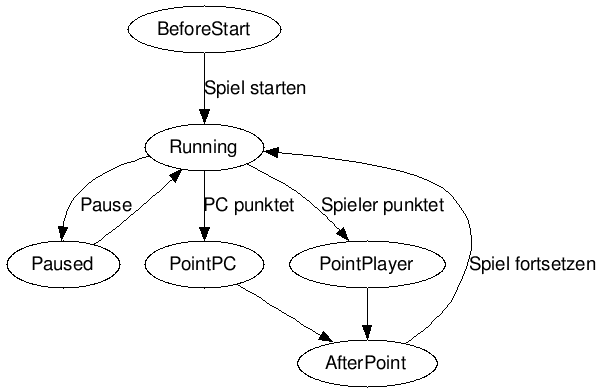
\includegraphics[width=0.33\textwidth]{fsm.png}
\caption{Spielzustands-Automat}
\end{figure}\\\\
Zur Umsetzung des Spiels müssen im wesentlichen Die vier Wände, der Ball und die Schläger gezeichnet werden. Des weiteren müssen das aktuelle Level (In Form von Schädeln) und die aktuelle Anzahl der Extra-Leben (als Herzen) angezeigt werden. Wird das Spiel gestartet, kann der Schläger mit der Maus gesteuert und der Ball mit Enter gestartet werden. Berührt der Ball einen Schläger muss je nach Geschwindigkeit des Schlägers die Flugbahn des Balls angepasst werden. Ebenfalls wird bei jeder Kollision ein zufälliger Sound abgespielt. \\
Verlässt der Ball das Spielfeld auf der Seite des Gegners, gewinnt der Spieler und der Schwierigkeitsgrad erhöht sich. Dies zeigt sich an einem schnelleren Ball und einem besser reagierenden Computergegner.\\
Verlässt der Ball das Spielfeld auf der Seite des Spielers, so wird ein Extra-Leben angezogen. Erreicht die Anzahl der Leben null, so gilt das Spiel als verloren und beginnt von vorne.